\documentclass[a4paper,12pt]{article} 

\usepackage[top = 2.5cm, bottom = 2.5cm, left = 2.5cm, right = 2.5cm]{geometry} 

% packages
\usepackage{amsmath, amsfonts, amsthm} % basic math packages
\usepackage{tikz} % for making illustrations
\usetikzlibrary{shapes.arrows, arrows, decorations.markings, positioning}
\usetikzlibrary{calc}
\usetikzlibrary{3d}
\usepackage{graphicx} % for importing images
\usepackage{xcolor} % more color options
\usepackage{colortbl}
\usepackage{multicol} % for making two-column lists
\usepackage{hyperref} % for hyperlinking
%\hypersetup{colorlinks=true, urlcolor=cyan,}
\usepackage{mathabx}
\usepackage{cleveref}
\usepackage{subfig}
\usepackage{array}
\usepackage{wrapfig}
\usepackage{bbm}
\usepackage{fancyhdr}
\usepackage{algorithm, algorithmicx, algpseudocode}
\usepackage{stmaryrd}
\usepackage{physics}


% The following two packages - multirow and booktabs - are needed to create nice looking tables.
\usepackage{multirow} % Multirow is for tables with multiple rows within one cell.
\usepackage{booktabs} % For even nicer tables.

% As we usually want to include some plots (.pdf files) we need a package for that.
\usepackage{graphicx} 

% The default setting of LaTeX is to indent new paragraphs. This is useful for articles. But not really nice for homework problem sets. The following command sets the indent to 0.
\usepackage{setspace}
\setlength{\parindent}{0in}

% Package to place figures where you want them.
\usepackage{float}

% The fancyhdr package let's us create nice headers.
\usepackage{fancyhdr}

% theorems, lemmas, examples, etc.
\newtheorem{theorem}{Theorem}[section]
% \newtheorem{corollary}{Corollary}[theorem]
% \newtheorem{lemma}[theorem]{Lemma}
\newtheorem{example}[theorem]{Example}
\newtheorem{lemma}[theorem]{Lemma}
\theoremstyle{definition}
\newtheorem{definition}{Definition}[section]
\theoremstyle{remark}
\newtheorem*{remark}{Remark}
\newtheorem*{solution}{Solution}

\def\mydefb#1{\expandafter\def\csname bf#1\endcsname{\mathbf{#1}}}
\def\mydefallb#1{\ifx#1\mydefallb\else\mydefb#1\expandafter\mydefallb\fi}
\mydefallb aAbBcCdDeEfFgGhHiIjJkKlLmMnNoOpPqQrRsStTuUvVwWxXyYzZ\mydefallb

\def\mydefb#1{\expandafter\def\csname cal#1\endcsname{\mathcal{#1}}}
\def\mydefallb#1{\ifx#1\mydefallb\else\mydefb#1\expandafter\mydefallb\fi}
\mydefallb aAbBcCdDeEfFgGhHiIjJkKlLmMnNoOpPqQrRsStTuUvVwWxXyYzZ\mydefallb

%% Change this to just the normal N,Z,R,C,P,E
\def\mydefb#1{\expandafter\def\csname bb#1\endcsname{\mathbb{#1}}}
\def\mydefallb#1{\ifx#1\mydefallb\else\mydefb#1\expandafter\mydefallb\fi}
\mydefallb CEGIKNPQRST\mydefallb

\newcommand{\half}{\frac{1}{2}}
\DeclareMathOperator{\sgn}{sgn}
\DeclareMathOperator*{\argmax}{arg\,max}
\DeclareMathOperator*{\argmin}{arg\,min}
\DeclareMathOperator{\prox}{prox}
\newcommand{\matlab}{\textsc{Matlab}}


%%%%%%%%%%%%%%%%%%%%%%%%%%%%%%%%%%%%%%%%%%%%%%%%
% 3. Header (and Footer)
%%%%%%%%%%%%%%%%%%%%%%%%%%%%%%%%%%%%%%%%%%%%%%%%

% To make our document nice we want a header and number the pages in the footer.

\pagestyle{fancy} % With this command we can customize the header style.

\fancyhf{} % This makes sure we do not have other information in our header or footer.

\lhead{\footnotesize CS 534:  Homework  \# 2}% \lhead puts text in the top left corner. \footnotesize sets our font to a smaller size.

%\rhead works just like \lhead (you can also use \chead)
\rhead{\footnotesize Scott (mtscot4)} %<---- Fill in your lastnames.

% Similar commands work for the footer (\lfoot, \cfoot and \rfoot).
% We want to put our page number in the center.
\cfoot{\footnotesize \thepage} 

\begin{document}
	
	
	%%%%%%%%%%%%%%%%%%%%%%%%%%%%%%%%%%%%%%%%%%%%%%%%
	%%%%%%%%%%%%%%%%%%%%%%%%%%%%%%%%%%%%%%%%%%%%%%%%
	
	%%%%%%%%%%%%%%%%%%%%%%%%%%%%%%%%%%%%%%%%%%%%%%%%
	% Title section of the document
	%%%%%%%%%%%%%%%%%%%%%%%%%%%%%%%%%%%%%%%%%%%%%%%%
	
	% For the title section we want to reproduce the title section of the Problem Set and add your names.
	
	\thispagestyle{empty} % This command disables the header on the first page. 
	
	\begin{tabular}{p{15.5cm}} % This is a simple tabular environment to align your text nicely 
		{\large \sc CS 534:  Machine Learning} \\
		Emory University \\ Fall 2024 \\ Prof. Eugene Agichtein \\
		\hline % \hline produces horizontal lines.
		\\
	\end{tabular} % Our tabular environment ends here.
	
	\vspace*{0.3cm} % Now we want to add some vertical space in between the line and our title.
	
	\begin{center} % Everything within the center environment is centered.
		{\Large \bf Homework \# 2} % <---- Don't forget to put in the right number
		\vspace{2mm}
		
		% YOUR NAMES GO HERE
		{\bf Mitchell Scott}\\ (mtscot4) % <---- Fill in your names here!
		
	\end{center}  
	
	\vspace{0.4cm}
	
	%%%%%%%%%%%%%%%%%%%%%%%%%%%%%%%%%%%%%%%%%%%%%%%%
	%%%%%%%%%%%%%%%%%%%%%%%%%%%%%%%%%%%%%%%%%%%%%%%%
	
	% Up until this point you only have to make minor changes for every week (Number of the homework). Your write up essentially starts here.
	
	\begin{enumerate}
		\item {\bf  Written(10 pts) Bias-Variance Trade-off of LASSO}
		While it is hard to write the explicit formula for the bias and variance of using LASSO, we can quantify the expected general trend. Make sure you justify the answers to the following questions for full points:
		\begin{enumerate}
			\item {\bf(Written) What is the general trend of the bias as $\lambda$ increases?}
			\begin{solution}
				The general trend for Lasso is as $\lambda$ increases, the bias increases. As $\lambda$ increases, that means that if there are more features, the $\norm{\beta}_1$ will increase, and that is scaled by $\lambda$, which is a very large number. This incentivises the model to include as few features as possible in very small amount. Using less features than needed, is the classic underfitting problem, so we have high bias. 
				
			\end{solution}
			\item {\bf (Written) What about the general trend of the variance as $\lambda$ increases?}
			\begin{solution}
				As $\lambda$ increases, the variance decreases. This makes sense as we have a simpler model with less parameter/ features that we are dealing with. This means that we cannot possible overfit, which is common with high variance situations. Since the model is simpler, then it is less data or problem dependent and can be used for other data sets rather easily.
			\end{solution}
			\item {\bf(Written) What is the bias at $\lambda = 0$?}
			\begin{solution}
				When $\lambda= 0$, we must recall that the regularization term $+\lambda\norm{\beta}_1$ becomes zero, so the loss function we are fitting is simpily the ordinary least squares problem, or Linear Regression model.
			\end{solution}
			\item {\bf(Written) What about the variance at $\lambda = \infty$?}
			\begin{solution}
				With $\lambda$ this high, that means we have a very biased model with very low variance. If there were any feature at all, then the $\norm{\beta}_1$ would be positive, and the loss function would be infinite. This means we cannot afford to imcorporate any features in our model, so we simply have the constant intercept as our model.
			\end{solution}
		\end{enumerate}
			
		\item{\bf Code+Written(40 pts) Spam classification using Naive Bayes and Standard Logistic Regression}
		\begin{enumerate}
			\item {\bf (Code) You will explore the effects of feature preprocessing and its impact on Naive Bayes and Standard (unregularized) logistic regression. Write the following functions to preprocess your data. You are free to use the \texttt{sklearn.preprocessing} module. Note that they functions should be independent of one another and should not build on each step/call each other. You should assume only the features are passed, in and not the target. These functions should accept numpy 2darray as input, return the preprocessed train and test set in numpy 2D array format (i.e., two return values)}.
				\begin{enumerate}
					\item {\bf  function \texttt{do\_nothing(train, test)} that takes a train and test set and does no preprocessing.}
					\item {\bf function \texttt{do\_std(train, test)} that standardizes the columns so they all have mean 0 and unit variance. Note that you want to apply the transformation you learned on the training data to the test data. In other words, the test data may not have a mean of 0 and unit variance.}
					\item {\bf function \texttt{do\_log(train, test)} that transforms the features using $\log(x_{ij} + 0.1)$ or a smoothed version of the natural logarithm.}
					\item {\bf function \texttt{do\_bin(train, test)} that binarize the features using $\bbI_{(x_{ij} >0)}$.  (Note that $\bbI$ denotes the indicator function). In other words, if the feature has a positive value, the new feature is a 1, otherwise, the value a 0.}
				\end{enumerate}

			\begin{solution}
				Implimented in \texttt{`q2.py'}.
			\end{solution}
			\item {\bf  (Code) Write a Python function \texttt{eval\_nb(trainx, trainy, testx, testy)} that fits a Naive Bayes model to the training. You can use \texttt{sklearn.naive\_bayes} module for this part. The function should accept as input numpy 2d arrays, and return a dictionary containing the accuracy and AUC for the training and test sets and the predicted probabilities for the test set: \\
				\texttt{return {"train-acc":
					train\_acc, "train-auc": train\_auc, "test-acc": test\_acc, "test-auc":
					test\_auc, "test-prob": test\_prob}}. \\
				The values for accuracy and AUC should be scalar
				numeric values, while test-prob should be a numpy 1-d array with the predicted probability for the positive class 1, for the test.}
			\begin{solution}
					Implimented in \texttt{`q2.py'}.
			\end{solution}
			\item {\bf (Written) Fit a Naive Bayes model to each of the four preprocessing steps above using the code in 2b. Each preprocessing should be performed independently (i.e., use each of the functions you created in 2a on the original dataset). Report the accuracy rate of and AUC of NB on the training and test sets across the 4 preprocessing steps in a table.}	
			\begin{solution}
				We compare the different preprocessing methods based on training and test accuracy and area under the ROC curve (auc) in Tab.  \ref{tab:nbresults}. As we see from the bolded numbers, we have the largest (either highest accuracy or highest auc, which is preferable) number in the logorithmic scaling, so it appears on these four metrics, \texttt{do\_log} is the best preprocessor for the Naive Bayes model using Spam classificiation.
				\begin{figure}[h]
					\centering
					\begin{tabular}{|c|cccc|}
						\hline
						&  \texttt{'train-acc'}&\texttt{'train-auc'}  & \texttt{'test-acc'} &  \texttt{'test-auc'}\\
						\hline\hline
						\texttt{do\_nothing}&  0.82561&  0.85096&0.81750  &0.83712  \\
						\texttt{do\_std}&  0.81627& 0.84305 & 0.81063 &0.83127  \\
						\texttt{do\_log}&{\bf0.83228}  & {\bf0.85573} & {\bf0.81875} & {\bf0.83795} \\
						\texttt{do\_bin}& 0.79860&0.82739  & 0.80063 &  0.82277\\
						\hline
					\end{tabular}
					\caption{Comparing the different preprocessing methods for Naive Bayes on the Spam Classification task. Bolded means the result is the highest of all methods in that metric.}
					\label{tab:nbresults}
				\end{figure}
				
			\end{solution}
			\item {\bf(Code) Write a Python function \texttt{eval\_lr(trainx, trainy, testx, testy)} that fits a ordinary (no regularization) logistic regression model. The function should return a dictionary containing theaccuracy and AUC for the training and test sets and the predicted probabilities for the test: \\
				
				\texttt{\{"train-acc": train\_acc, "train-auc": train\_auc, "test-acc": test\_acc, "test-
					auc": test\_auc, "test-prob": test\_prob\}}.\\
				 Note that the values for accuracy and AUC should be scalar numeric values, while test-prob should either be a numpy 1-d array with the predicted probability of positive class 1 for the test set. The output will be the same format as 2b.}
			\begin{solution}
					Implimented in \texttt{`q2.py'}.
			\end{solution}
			\item {\bf(Written) Fit ordinary (no regularization) logistic regression model with each of the four preprocessing steps above using the code in 2d. Report the accuracy rate and AUC on the training and test sets for the 4 preprocessing steps in a table}
			\begin{solution}
				We compare the different preprocessing methods based on training and test accuracy and area under the ROC curve (auc) in Tab.  \ref{tab:lrresults}. As we see from the bolded numbers, we have the largest number in the logorithmic scaling, so it appears on these four metrics, \texttt{do\_log} is the best preprocessor for the Logistic Regression model using Spam classificiation.
				\begin{figure}[h]
					\centering
					\begin{tabular}{|c|cccc|}
						\hline
						&  \texttt{'train-acc'}&\texttt{'train-auc'}  & \texttt{'test-acc'} &  \texttt{'test-auc'}\\
						\hline\hline
						\texttt{do\_nothing}& 0.93398& 0.92817& 0.92063& 0.91273 \\
						\texttt{do\_std}& 0.93464& 0.92871& 0.92063&0.91274 \\
						\texttt{do\_log}&{\bf0.94431}& {\bf0.94111}&{\bf0.93313}&{\bf0.92677}\\
						\texttt{do\_bin}& 0.93898& 0.93417&0.92500& 0.91691\\
						\hline
					\end{tabular}
					\caption{Comparing the different preprocessing methods for Logistic Regression on the Spam Classification task. Bolded means the result is the highest of all methods in that metric.}
					\label{tab:lrresults}
				\end{figure}
				Additionally, it is noted that the do nothing preconditioning method resulted in a `did not converge' error using LBFGS up to 5000 iterations, so it was rerun with Newton-CSG as the iterative solver, where there was convergence for all of the preprocessing steps. While the exact accuracies are slightly different, they are the same as the LBFGS method for up to 4 decimal places, and the overall trends of logarithmic preprocessing still reigns supreme. 
				Lastly, it is imperative to note that Logistic Regression did between 10 and 15 \% better than Naive Bayes for the same data set.
				\end{solution}
			\item {\bf(Written) Plot the receiver operating characteristic (ROC) curves for the test data. You should generate 3 plots:}
				\begin{itemize}
				\item {\bf One plot containing the 4 Naive Bayes model curves representing each of the preprocessing steps.
				\item One plot containing the 4 logistic regression model curves representing each of the preprocessing
				steps.
				\item One plot containing the best Naive Bayes model and the best logistic regression model curve. }
				\end{itemize}
			\begin{solution}
				\begin{figure}
					\centering
					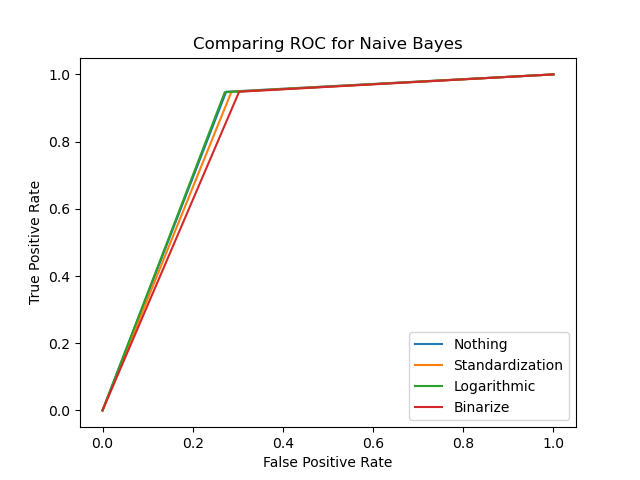
\includegraphics[width=0.7\linewidth]{../nb}
					\caption{Comparing the ROC curves for different preprocessing features for Naive Bayes.}
					\label{fig:nb}
				\end{figure}
		
			\begin{figure}
				\centering
				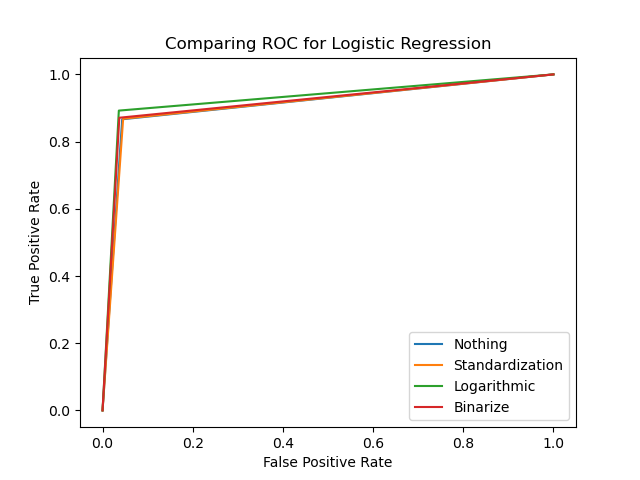
\includegraphics[width=0.7\linewidth]{../lr}
				\caption{Comparing the ROC curves for different preprocessing features for Logistic Regression.}
				\label{fig:lr}
			\end{figure}
			\begin{figure}
				\centering
				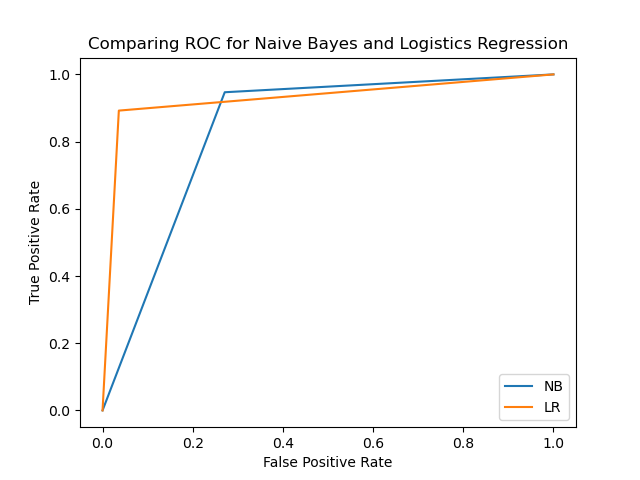
\includegraphics[width=0.7\linewidth]{../best}
				\caption{Using the best preprocessing function (logarithmic), we then compare how Naive Bayes and Logistic Regression perform on this dara by the ROC curve metric.}
				\label{fig:best}
			\end{figure}
			
			There does appear to be something weird with these ROC curves as there is only three points. I feel that I have done something wrong there as they should be more smooth.
			\end{solution}
			\item {\bf (Written) Given your results in 2c, 2e, and 2f, discuss how the preprocessing affects the models (Logistic and Naive Bayes) with regards to ROC, AUC, and accuracy. Also, comment on how Naive Bayes performance compares with logistic regression}
			\begin{solution}
			We notice that from the plots and tables that the best preprocessing method is logarithmic, then binary, then standarization barely surpassing doing nothing. We also observe that the logistic regression is about 10-15\% more accurate than naive Bayes.
				
			\end{solution}
		\end{enumerate}
		\item {\bf (50 pts) Exploring Model Selection Strategies for Logistic Regression with Regularization
			We will be using the SPAM dataset from the previous part for this problem. You can preprocess the data
			however you see fit, either based on the results of the previous problem or by introducing another
			preprocessing method. The only requirement is that it is consistent throughout the rest of this problem.
			For this problem, you are not allowed to use the \texttt{sklearn.model\_selection} module. All the specified functions should be in the file \texttt{‘q3.py’}.}
	
		\begin{enumerate}
			\item {\bf (Written) How did you preprocess the data for this problem? Why?}
			\begin{solution}
				Based on the results up above, the data was preprocessed using the logarithmic scaling. This was preformed exactly as it was in question 2. We initially separated the train and test data from the different .dat files. Then we did log scaling on the train and test $x$ values, then we concatenated the \texttt{trainx, testx} and \texttt{trainy,testy}.
			\end{solution}
			\item {\bf (Code) Implement the Python function \texttt{generate\_train\_val(x, y, valsize)} that given the validation size splits the data randomly into train and validation splits. The function should return a dictionary \\
				\texttt{return \{"train-x": tr\_x, "train-y": tr\_y, "val-x": ts\_x, "val-y": ts\_y\}.}\\ 
				The values for \texttt{‘train-x’} and \texttt{‘val-x’} are expected to be numpy 2d arrays of the same dimension as $x$, and split into the associated training and validation features. The values for \texttt{‘train-y’} and \texttt{‘val-y’} are expected to be a subset
				of $y$ split accordingly. Note that each time this function is run, the splits could be different.}
			\begin{solution}
				Implimented in \texttt{`q3.py'}.
			\end{solution}
			\item {\bf (ridgeCode) Implement the Python function \texttt{generate\_kfold(x, y, k)} that given the $k$, will split the data into $k$-folds. The function should return a single numpy 1-d array, containing the $k$ that each item index it belongs to (e.g., array([0,1,2,. . . ,2,1,1])) for $k=3$, which indicates item 0 belongs to fold 0, and item 1 belongs to fold 1, etc.}
			\begin{solution}
				Implimented in \texttt{`q3.py'}.
			\end{solution}
			\item {\bf (Code) Implement the Python function\texttt{eval\_holdout(x, y, valsize, logistic)} which takes in the input (e.g., 3000 training samples from spam.train.dat), the input labels, and the validation size and (1) uses 3b to split $x$ and $y$ into train and validation, and (2) evaluates the performance using the logistic regressionmodel passed in as . You can assume the logistic regression classifier will be created using \texttt{sklearn.linear\_model.LogisticRegression} and initialized before passed to your method, so you can invoke it as usual. Your function should return a dictionary containing the accuracy and AUC for the training and validation sets using keys \texttt{‘train-acc’, ‘train-auc’, ‘val-acc’, ‘val-auc’}.}
			\begin{solution}
				Implimented in \texttt{`q3.py'}.
			\end{solution}
			\item {\bf (Code) Implement function \texttt{eval\_kfold(x, y, k, logistic)} which takes in number of folds $k$, (1) uses 3c to split the data, and (2) evaluates the performance using the input classifier logistic instantiated as logistic regression model. You can assume the logistic regression classifier will be created using \texttt{sklearn.linear\_model.LogisticRegression}. Your function should return a dictionary containing the accuracy and AUC for the training and validation sets using the following keys: \texttt{‘train-acc’, ‘train-auc’, ‘val-acc’, ‘val-auc’}. The accuracy and AUC for this part should be a averaged across the $k$ folds.}
			\begin{solution}
				Implimented in \texttt{`q3.py'}.
			\end{solution}
			\item {\bf (Code) Implement the Python function \texttt{eval\_mccv(x, y, valsize, s, logistic)} that takes in the validation size and the sample size $s$ and uses the Monte Carlo cross-validation approach with $s$ rounds (i.e., use the validation/hold-out technique from 3d, $s$ times). The output should be the same format as 3e.}
			\begin{solution}
				Implimented in \texttt{`q3.py'}.
			\end{solution}
			\item {\bf (Written) Fit Ridge and LASSO using the $K$-fold cross validation approach with $k = 5, 10$, and varying alpha (regularization weight). Report the best setting (combination of $k$ and regularization weight alpha)}
			\begin{solution}
				First, it is important to know that when we are building these, the \texttt{C} parameter is the `inverse of regularization strength' from the SciKit-Learn documentation. So as opposed to putting $\alpha$ as the regularization parameter, we have to set it up so that $C := \frac{1}{\alpha}$. 
				
				Since We don't know where to start, we use $C=1$, which is the default for the Logistic Regression Model. Additionally, to make everything fairer, we set the solver to \texttt{`liblinear`}, as that is the first solver that works on both $\ell^1$ and $\ell^2$ regularization. Below are the results.
				\begin{figure}[h]
				\centering
				\begin{tabular}{|c|cccc|}
					\hline
					&  \texttt{'train-acc'}&\texttt{'train-auc'}  & \texttt{'test-acc'} &  \texttt{'test-auc'}\\
					\hline\hline
					Ridge, $k=5$& 0.94253& 0.93799 &0.93928, & 0.93452\\
					Ridge, $k=10$& {\bf0.94334}& {\bf0.93902}& {\bf0.94061}& {\bf0.93618}\\ \hline
					Lasso, $k=5$&0.94515& {\bf0.94110}& {\bf0.94146}& {\bf0.93695}\\ 
					Lasso, $k=10$&  {\bf0.94518}& 0.94108 & 0.94027& 0.93624\\ 
					\hline
				\end{tabular}
				\caption{Comparing the variations of Logistic Regression regularization and $k$ for $k-$folds  on the Spam Classification task. Bolded means the result is the highest of all methods in that metric.}
				\label{tab:kfoldresults1}
			\end{figure}
			We see in Tab. \ref{tab:kfoldresults1} that for Ridge regression, $k=10$ is better for every metric, but for Lasso regression $k=5$ is better especially for the test data.
			
			Lastly, to get varying $\alpha$, we ran a loop for every $\alpha$ value from 0 to 1 up to three decimimal places.
			This information uses \texttt{test-acc} as the metric we are comparing. 
				\begin{figure}[h]
				\centering
				\begin{tabular}{|c|cc|}
					\hline
					 Model &\texttt{'test-acc'} &$\hat{\alpha}$ \\
					\hline\hline
					Ridge, $k=5$& 0.94278 & $\hat{\alpha} = 0.248$\\
					Ridge, $k=10$& 0.94293&$\hat{\alpha} = 0.530$\\
					\hline
					Lasso, $k=5$&0.94260&$\hat{\alpha} = 0.271$\\
					Lasso, $k=10$&   0.94382&$\hat{\alpha} = 0.992$\\
					\hline
				\end{tabular}
				\caption{Up to 3 decimal places, these are the best $\hat{\alpha}$ values, which produce the highest \texttt{`test-acc'} in the respective models}
				\label{tab:kfoldresults2}
			\end{figure}
			As we can see from Tab. \ref{tab:kfoldresults2}, depending on the model and $k$ value, we have very different $\hat{\alpha}$ values, but similar, high test-accuracy.
			\end{solution}
			\item {\bf (Written) Fit Ridge and LASSO using the Monte Carlo Cross-validation (MCCV) approach with $s = 5, 10$ rounds and different valsize ratios, and varying alpha (regularization weight). Report the best setting (combination of valsize, $s$, alpha).}
			\begin{solution}
				Just like above, we iterate through $\alpha$ values and then make the Logistic Regression model for both Ridge and Lasso with $C = \frac{1}{\alpha}$. We iterate through all of the values for alpha between 0 and 1 up to three decimal places. Additionally, we have the \texttt{valsize} parameter to iterate through as well, so I set the possible values to be 46, 92, 138, which corresponds to 10, 20, and 30 \% of the total dataset ($n=4601$). 
					\begin{figure}[h]
					\centering
					\begin{tabular}{|c|ccc|}
						\hline
						Model &\texttt{'test-acc'} &$\hat{\alpha}$ & Test Data \%\\
						\hline\hline
						Ridge, $s=5$& 0.97826 & $\hat{\alpha} = 0.950$ &20\% \\
						Ridge, $s=10$& 0.96957&$\hat{\alpha} = 0.390$ &20\%\\
						\hline
						Lasso, $s=5$&0.98261&$\hat{\alpha} = 0.569$ &20\%\\
						Lasso, $s=10$&   0.97174&$\hat{\alpha} = 0.332$& 20\%\\
						\hline
					\end{tabular}
					\caption{Up to 3 decimal places, these are the best $\hat{\alpha}$ values, which produce the highest \texttt{`test-acc'} in the respective models with what percent of the data was test data.}
					\label{tab:mccvresults2}
				\end{figure}
				We see many interesting things in Tab. \ref{tab:mccvresults2}, namely that when $s=5$, the model is about 1\% more accurate. Additionally, the 80/20 train/test split appears to universally be the best way to partitiion the data. However, I am slightly doubious about these results as we see almost 100\% accuracies, which is making me question if we are possible mixing our test and training data and memorizing it.
			\end{solution}
			\item {\bf (Written) Using the best parameters identified in 3g and 3h, re-train the regularized logistic regression models (Ridge, Lasso) using all the training data and report the performance on the test set in terms of AUC and accuracy in a table. You should have 4 models to compare: Ridge and Lasso trained using best parameters from k-fold and Ridge and Lasso using best parameters from MCCV. Compare how the model selection techniques compare to one another w.r.t. AUC and accuracy, predicted vs. actual test error, and computational complexity (running time).}
			\begin{solution}
				\begin{figure}[h]
					\centering
					\begin{tabular}{|c|cccc|}
						\hline
						Model &\texttt{'train-acc'} &\texttt{'train-auc'}  & \texttt{'test-acc'}& \texttt{'test-auc'} \\
						\hline\hline
						Ridge, k-fold& 0.94388& 0.93969&0.94031& 0.93583 \\
						Lasso, k-fold& 0.94492& 0.94089& 0.94102 & 0.93719\\
						\hline
						Ridge, MCCV&0.94359&0.93933 &0.93478&0.92793\\
						Lasso, MCCV&   0.94447&0.94947&0.92609& 0.91980\\
						\hline
					\end{tabular}
					\caption{Comparing the Optimal Parameters for k-fold and MCCV using Ridge and Lasso Logistic Regression.}
					\label{tab:mccvresults1}
				\end{figure}
				We see from the Tab. \ref{tab:mccvresults1}, that Lasso is better than Ridge in both settings and k fold is better than the respective mccv value. In terms of running time, both models took about 1 second to run. Additionally k-fold has a better predicted vs actual test error.
			\end{solution}
		\end{enumerate}
		
	\end{enumerate}
	
	
	
	
	\section*{Acknowledgements}
	I would like to acknowledge that I didn't work with any other CS 534, nor did I attend TA or Professor OH this week.
	
\end{document}
